\documentclass[a4paper,12pt]{article}

\usepackage{rotating}
\usepackage[top=1.25in, bottom=1.25in, left=1.25in, right=1.25in]{geometry}
\usepackage{graphicx}
\usepackage[numbers,square,sort&compress]{natbib}
\usepackage{setspace}
\usepackage[cdot,mediumqspace,]{SIunits}
\usepackage{caption}
\usepackage{subcaption}
\usepackage{mathtools}
\usepackage{authblk}
\usepackage{float}
\usepackage{wrapfig}
\renewcommand{\thesubsection}{\thesection.\alph{subsection}}
\providecommand{\e}[1]{\ensuremath{\times 10^{#1}}}
\newcommand*\lap{\mathop{}\!\mathbin\bigtriangleup}

\begin{document}
\onehalfspacing
\title{Special Functions and Solving the Heat Equation for a Cold Cylinder}
\author{Natalie Price-Jones, 999091021}
\date{4 December 2014}
\affil{\small{natalie.price.jones@mail.utoronto.ca}}
\maketitle

\section{Question 1}
\begin{table}[H]
  \centering
  \begin{tabular}{|c||c||c||c||c|}
    \hline
    Factorial & math.factorial & Recursive & Stirling & Memoization\\
    \hline
    \hline
    10! & $3.0\e{-6}$ & $2.2\e{-5}$& $8.0\e{-6}$ & $3.7\e{-6}$\\
    \hline
    100! & $1.6\e{-5}$ & $2.1\e{-4}$ & $1.0\e{-6}$ & $4.0\e{-6}$\\
    \hline
    500! & $1.2\e{-4}$ & $1.0\e{-3}$ & Overflowed & $2.2\e{-5}$\\
    \hline
    1000! & $5.0\e{-4}$& Recursion exceeded & Overflowed & $3.9\e{-5}$\\
    \hline
  \end{tabular}
  \caption{}
\end{table}

It is obvious from this table that math.factorial is consistently faster than any function I write. This is because the math module relies on precomplied C libraries, inherently faster to run than interpreted languages like Python. In addition, math.factorial uses a divide and conquer method to compute factorials, reducing the time needed to evaluate.

When my first recursive function attempted to evaluate 1000!, it failed because it exceeded the maximum recursion depth allowed for a recursive function. Essentially, it went too many layers into itself. Initially memoization has the same problem, though of course once a sufficient number of lower factorials were saved, evaluating 1000! did not exceed the recursion depth. The Stirling approximation was by far the fastest of the three methods, but it was only successful in evaluation $\ln(1000!)$. This value could not be converted back to 1000! without an overflow error.

\textbf{part c)} One obvious advantage of memoization to compute factorials is that it extends the capabilities of our recursive function far beyond its normal range. However, these results are lost when the program is restarted, so the memoized data must be reevaluated each time the program is run. This shortcoming could be overcome by saving the results of the factorial computation and reading them in each time the program starts, appending new values to the end of the file as they are computed. This would overcome the obvious disadvantage of memoization and add only a short slow-down when the file is loaded in.

\textbf{part d)} For the remainder of the coding, I will be using the memoization function, as it is by far the fastest and can be used to evaluate larger factorials.

\section{Question 2}

\textbf{part b)}

\begin{figure}[H]
\centering
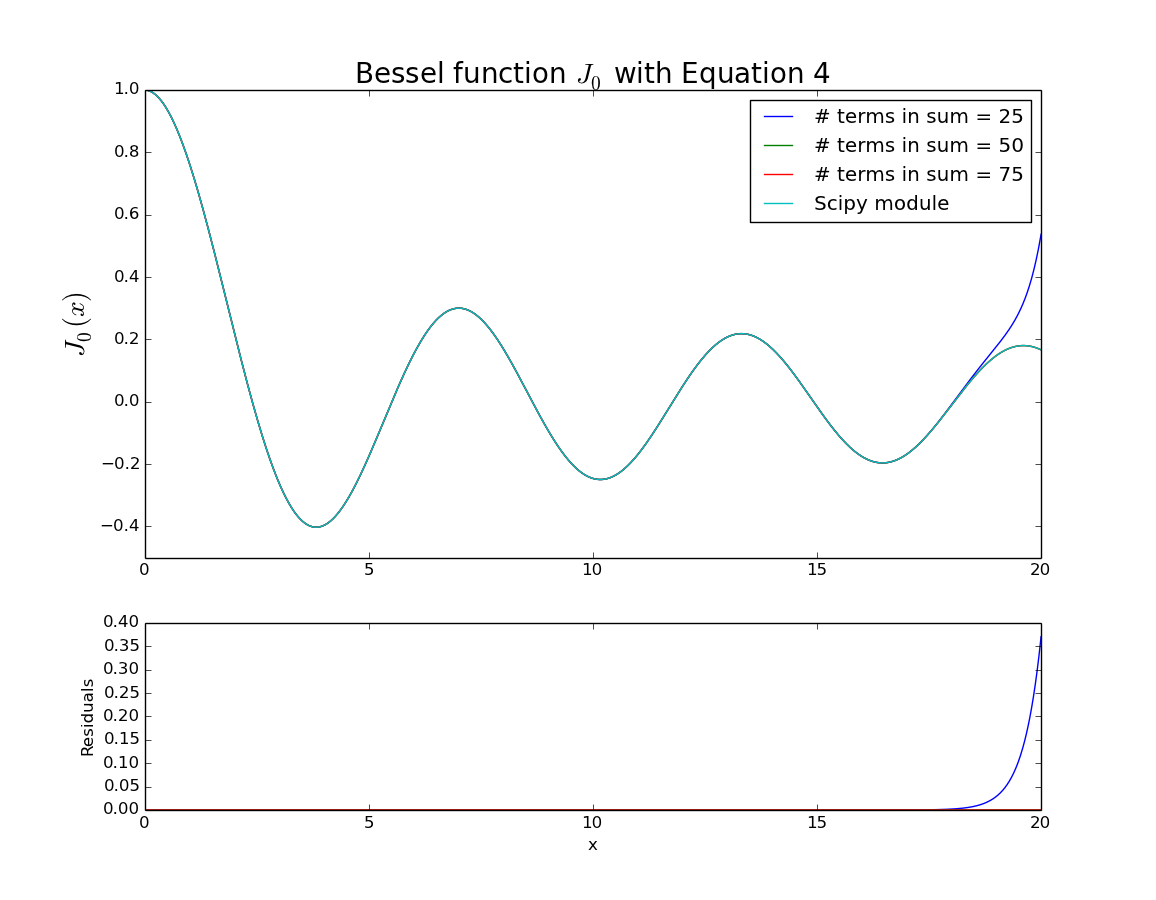
\includegraphics[width = \linewidth]{indepq2b.png}
\caption{}
\label{fig:q2b}
\end{figure}

\textbf{part c)}

\begin{figure}[H]
\centering
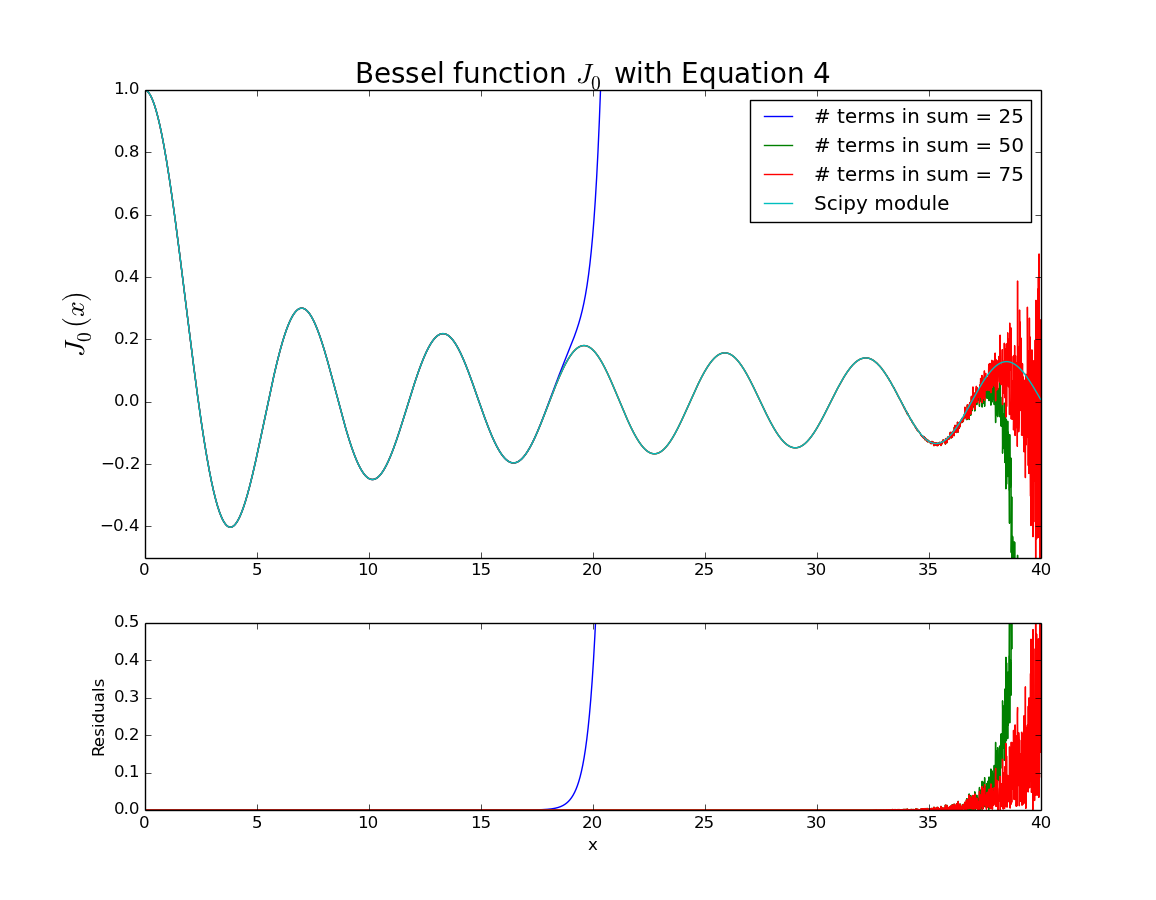
\includegraphics[width = \linewidth]{indepq2c.png}
\caption{}
\label{fig:q2c}
\end{figure}

\textbf{part d)}

\begin{figure}[H]
\centering
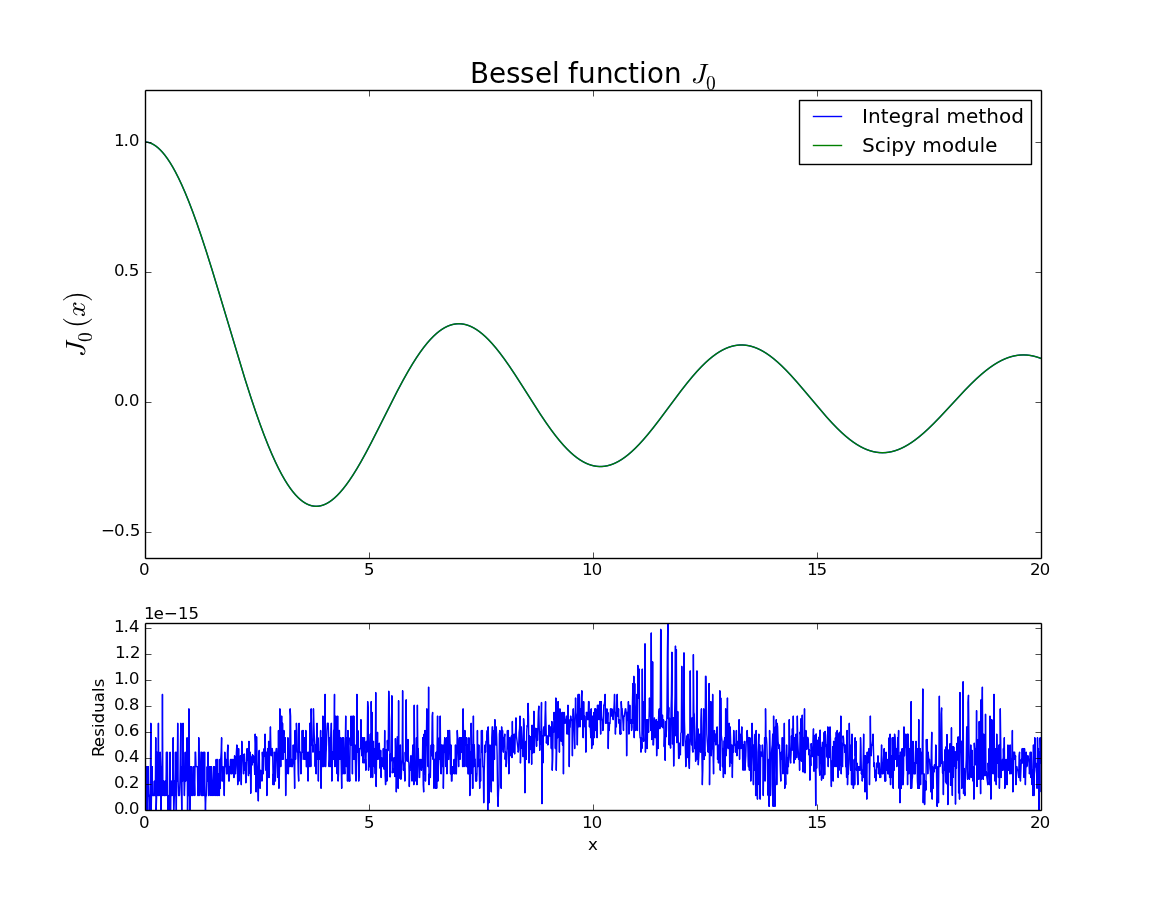
\includegraphics[width = \linewidth]{indepq2d.png}
\caption{}
\label{fig:q2d}
\end{figure}

\textbf{part e)} For the remainder of the code, I plan to use the integral equation for the Bessel function:

\begin{equation}
J_n(x) = \frac{1}{\pi}\int_0^{\pi}\cos(n\tau - x\sin(\tau)) d\tau,\nonumber
\end{equation} 
%
since this is quicker and easier to evaluate than an arbitrarily large sum, and matches our expected result (the scipy module) very well.

\textbf{part f)}

\begin{figure}[H]
\centering
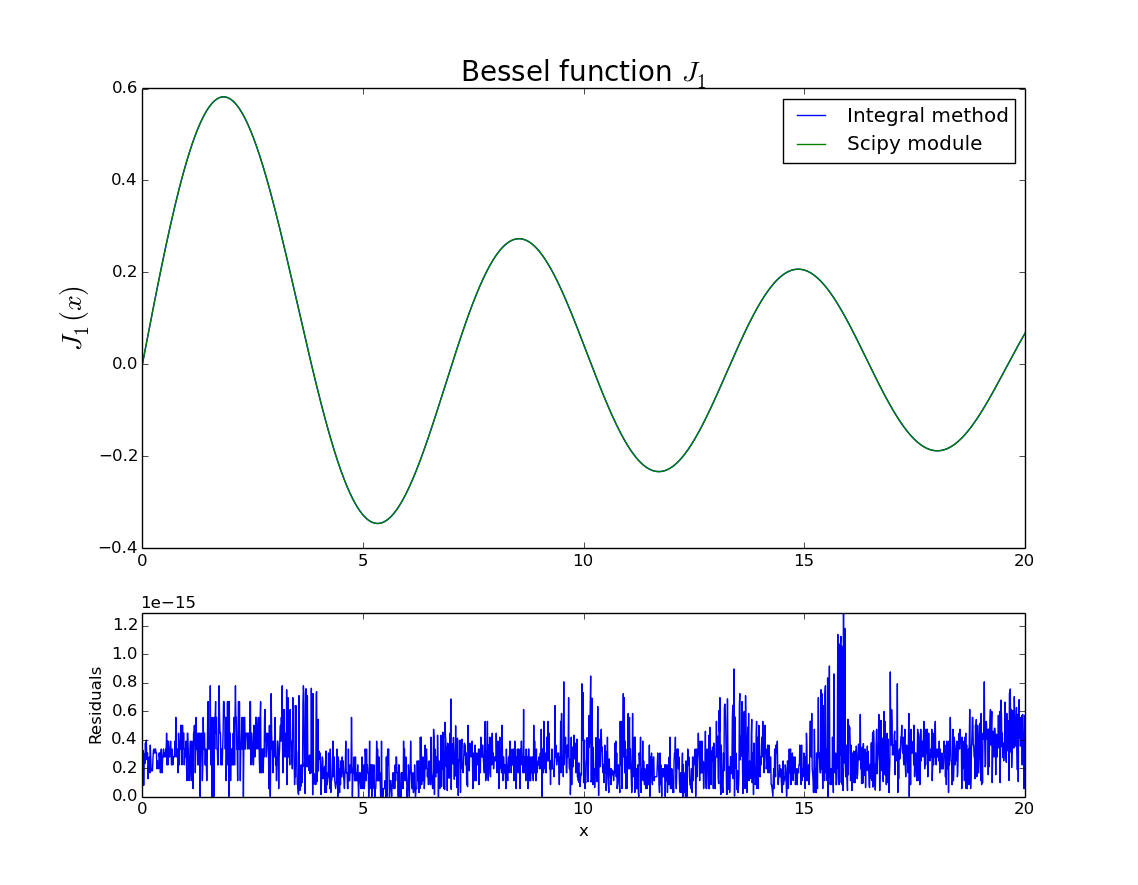
\includegraphics[width = \linewidth]{indepq2f.png}
\caption{}
\label{fig:q2f}
\end{figure}

\section{Question 3}

\textbf{part a)}

The required accuracy was $1\e{-5}$\\

\textbf{part b)}

\begin{table}[H]
  \centering
  \begin{tabular}{|c||c||c|c|}
    \hline
    Zero Index & Approximation Scheme & scipy.special.jn\_zeros & Difference\\
    \hline
    \hline
    5 & 14.9226 & 14.9309 & $8.3\e{-3}$\\
    \hline
    50 & 156.2942 & 156.2950 & $7\e{-4}$\\
    \hline
    500 & 1570.0109 & 1570.0110 & $8\e{-5}$\\
    \hline
  \end{tabular}
\end{table}

Obviously our approximation is best for large values of the zero index.

\section{Question 4} 

\begin{figure}[H]
\centering
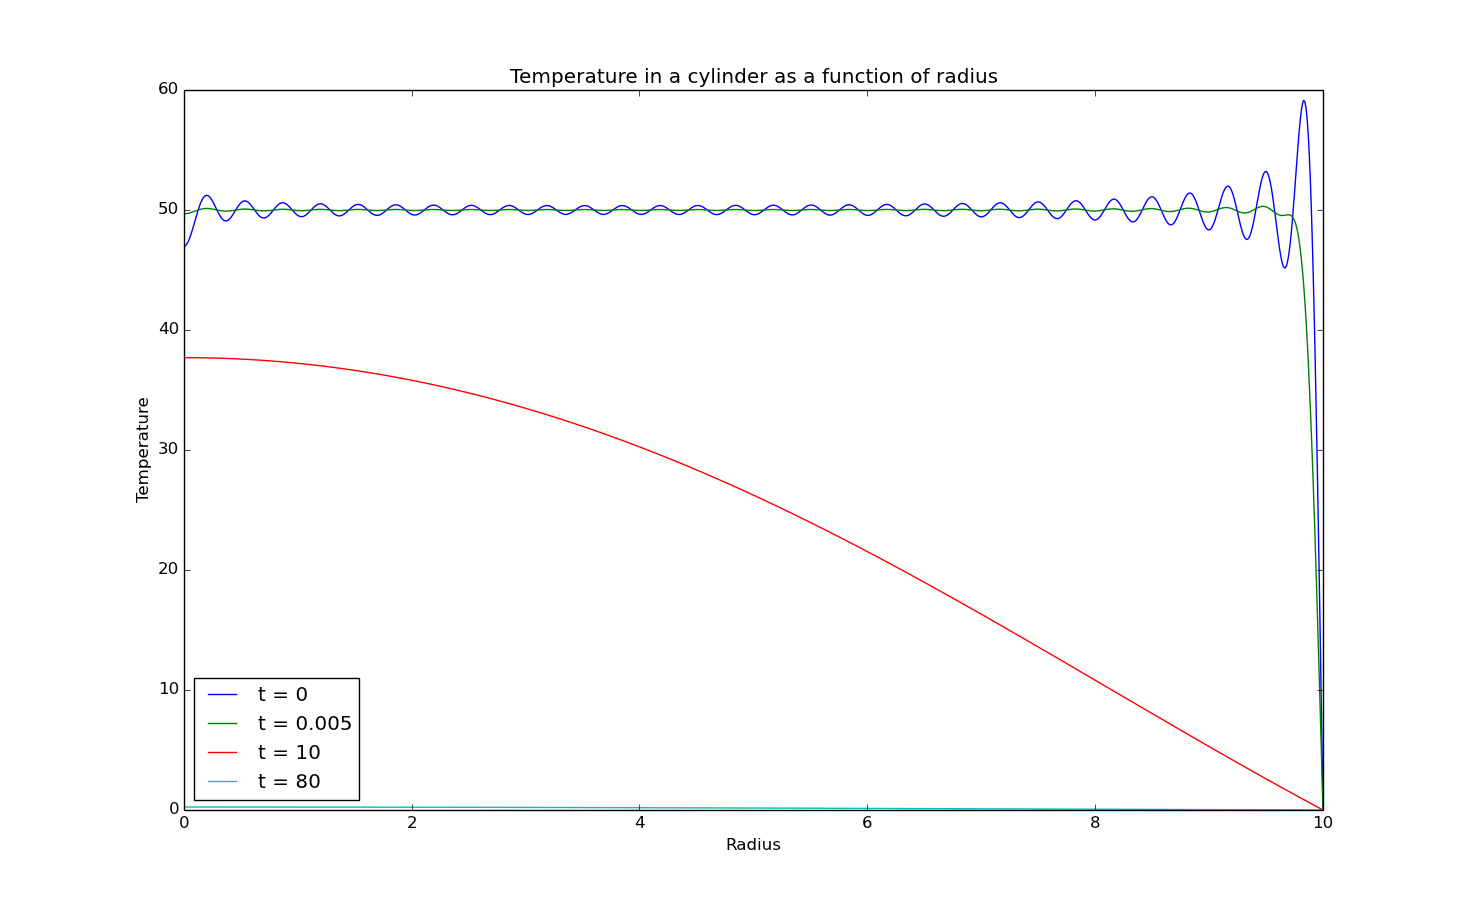
\includegraphics[width = \linewidth]{indepq4.png}
\caption{}
\label{fig:q4}
\end{figure}

At time 0, the temperature profile does not obey the initial conditions of the problem. This is because we are forced to truncate the solution to a finite number of terms in the sum. We are trying to use an oscillatory function to model a step function. We saw this exact sort of problem in a past lab when we tried to model a square wave with a Fourier series. As time goes on, the function smooths in the way we would expect. Further more, the total temperature decreases everywhere over time as expected, with low temperature regions moving inward from the outer edge where the temperature is fixed.

\end{document}
